

\documentclass[12pt,a4paper,oneside]{report}

\usepackage{titlesec}
\usepackage{geometry}
 \geometry{
 a4paper,
 top=35mm,
bottom=30mm,
bindingoffset=0.0in
 }
\pagenumbering{arabic} 

\usepackage{graphicx}
\usepackage{booktabs, chemformula}

\pagestyle{headings}

\newcommand{\dspaceon}{\renewcommand{\baselinestretch}{1.3}\large\normalsize}
\newcommand{\dspaceoff}{\renewcommand{\baselinestretch}{1}\large\normalsize}

\graphicspath{ {E:/faculta/Master/DissertationProject/images/} }

\usepackage{titlesec, blindtext, color}
\definecolor{gray75}{gray}{0.75}
\newcommand{\hsp}{\hspace{20pt}}
\titleformat{\chapter}[hang]{\Large\bfseries}{\thechapter\hsp\textcolor{gray75}{$|$}\hsp}{0pt}{\Large\bfseries}
\titleformat{\section}{\normalfont\large\bfseries}{\thesection}{1em}{}
\begin{document}
\begin{titlepage}
%\newgeometry{left=20mm,right=20mm,top=2.5cm,bottom=2cm}


\thispagestyle{empty}
\setlength\headheight{0pt} 
\begin{center}


\hfill 
\includegraphics[width=0.45\linewidth]{oxlogo.jpg}            


        \vspace{3cm}
        {\LARGE Computer Science and Engineering Department\\
"Politehnica" University of Timisoara \par}
        \vspace{3cm}

        {\Large\bfseries An analysis of the relationship between structural and logical\\ dependencies in software systems \par}
        
        \vspace{3cm}
        {\Large\itshape Adelina Diana Stana\par}
        \vspace{0.25cm}

\vspace{1cm}
Coordinated by\par
Assoc Prof.~Ioana \textsc{Sora}\par
\vspace{1.5cm}
\large
\today

\end{center}

\clearpage
\restoregeometry
\end{titlepage}



\tableofcontents
\newpage
\begin{abstract}
Software systems are continuously in change. Changes can be triggered by new features, defects, new technologies, system refactoring for maintainability \cite{ct1}.All of the actions from above have a direct impact on the structural and logical dependencies of the system \cite{ct8}, \cite{ct6}.\\Studying only the structural dependencies of the system is not enough to get a clear overview of the dependencies in the system . For more precise results is needed a study that combines structural dependencies and logical dependencies. We have analysed 17 open-source software systems of different sizes to investigate the overlappings between structural dependencies and logical dependencies. Furthermore, we have investigated the impact of different factors when building logical dependencies.\\The results from our analysis show that a significant number of structural dependencies are also logical but this number is influenced by the method of calculating the logical dependencies.
\end{abstract}
\newpage
\chapter{Introduction}
A dependency is created by two elements that are in a relationship and indicates that an element of the relationship, in some manner, depends on the other element of the relationship \cite{ct2}, \cite{ct3}. \\There are several types of relationships between source code entities, a method can call another class method, a class extends another class, all those create structural dependencies between classes (a.k.a syntactic dependencies or structural coupling) \cite{ct4}.\\In software engineering, co-evolution represents the phenomenon through one component changes in response to a change in another component \cite{ct6}, \cite{ct5}. Those changes can be found in the software history. Logical dependencies (a.k.a logical coupling) are the result of software history analysis and can reveal relationships that are not always present in the source code (structural depencencies)  Figure \ref{fig:fig1} .
\begin{figure}[h]
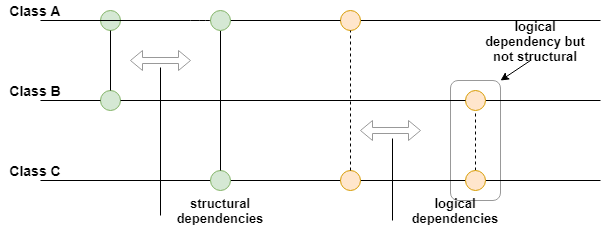
\includegraphics[scale=0.45]{fig1.png}
\caption{Relationships between structural and logical dependencies }
\label{fig:fig1}
\centering
\end{figure}
\begin{figure*}[h]
\centering
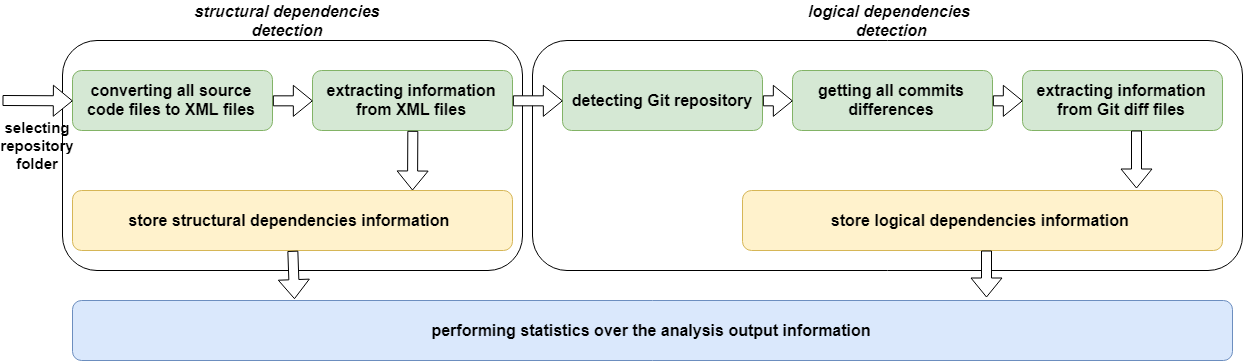
\includegraphics[width=\textwidth]{fig3.png}
\caption{Processing phases}
\label{fig:fig3}
\end{figure*}
\section {State of the art}

\section{Purpose of the project}
Lucrarea se incheie cu un capitol de concluzii.


\chapter{Theoretical aspects}

\section{Software dependencies}
In order to build structural and logical dependencies we have developed a tool that takes as input the source code repository and builds the required software dependencies . The workflow can be delimited by three major steps as it follows (Figure \ref{fig:fig3}):\\ \\
\textit{\textbf{Step 1:} Extracting structural dependencies.}\\
\textit{\textbf{Step 2:} Extracting logical dependencies.}\\
\textit{\textbf{Step 3:} Processing the information extracted.}

\section{Structural dependencies}
Even though in some of the cases if class A depends on class B , changes in class B can produce changes in class A, but not the other way around \cite{ct5} . There are some cases in which if class A depends on class B,  changes in class B can produce changes in class A and viceversa. So we will consider structural dependencies as bidirectional relationships, "class A depends on class B" and "class B depends on class A". The choice of building bidirectional relationships is also motivated by the fact that we cannot establish for the moment the direction of the logical dependencies of the system. So in order to have a omogeninty between the logical and structural dependencies analysis results, we will take both of the relationships types as bidirectional.
In this step the entire source code folder is scanned and only source code files are extracted in order to convert them into XML files (a.k.a  Extensible Markup Language files) through calls to an external tool called srcML \cite{ct9}. All the information about classes, methods, calls to other classes are afterwards extracted from the XML files.

\section{Logical dependencies}
The versioning system contains the long-term change history of every file. Each project change made by an individual at certain point of time is contained into a commit \cite{ct7}. All the commits are stored in the versioning system cronologicaly and each commit has a parent. The parent commit is the baseline from which development began, the only exeption to this rule is the first commit which has no parent. We will take into consideration only \textit{commits that have a parent} since the first commit can include source code files that are already in development (migration from one versioning system to another) and this can introduce reduntant logical links \cite{ct8} .The tool looks through the main branch of the project and gets all the existing commits, for each commit a diff against the parent will be made and stored.\\ Finally after all the differences files are stored , all the files are parsed and logical dependencies are build. In addition , the number of files changed in a commit can influence the logical dependencies. A relatively big number of files changed can indicate a merge of all changes from another branch as a single commit. This can lead to a number of logical dependencies that are redundant since the files are not actualy changing in the same time.The logical dependencies are splitted into three categories :\\
\textit{\textbf{Category 1:} Dependencies found in commits with less than 5 source code files changed.}\\
\textit{\textbf{Category 2:} Dependencies found in commits with more than 5 files changed but less than 20. }\\
\textit{\textbf{Category 3:} Dependencies found in commits with more than 20 files.}

Also for each category two dependencies analysis will be made:
\textit{\textbf{A:} Considering comments  as valid changes.}
\textit{\textbf{B:} Considering comments  as redundant changes. }
In the second case if class A and class B change together but the only change found is a comment change then between class A and B will not be set logical dependency.

\chapter{Tool for measuring software dependencies}

\chapter{Implementation details}
\section{Software dependencies}
\section{Logical dependencies}

\chapter{Tool usage}

\chapter{Experimental results}
In this study, we have made a set of statistical analysis on a set of open-source projects in order to extract the structural and logical dependencies between classes \cite{ct5}, \cite{ct8} . Table \ref{table:1} illustrates all the systems studied. The 1st column shows the projects IDs; 2nd column shows the project name; 3rd column shows the number of classes extracted; 4th column shows the number of commits from the main branch of each project and the 5th shows the language in which the project was developed.

\begin{table}[h]
  \centering
  \begin{tabular}{@{}ccccc@{}}
    \toprule
    ID  & Project    & Nr. of classes & Nr. of commits& Type\\
    \midrule
 \ch{1}	&	urSQL	&	41	&	89	&	java	\\
 \ch{2}	&	JavaCoder	&	5	&	11	&	java	\\
 \ch{3}	&	jbandwidthlog	&	14	&	54	&	java	\\
\ch{4}	&	sjava-logging	&	18	&	62	&	java	\\
\ch{5}	&	daedalum	&	66	&	29	&	java	\\
\ch{6}	&	prettyfaces	&	236	&	207	&	java	\\
\ch{7}	&	jbal	&	102	&	113	&	java	\\
\ch{8}	&	guavatools	&	237	&	85	&	java	\\
\ch{9}	&	monome-pages	&	240	&	280	&	java	\\
\ch{10}	&	kryo	&	309	&	743	&	java	\\
\ch{11}	&	bitlyj	&	21	&	81	&	java	\\
\ch{12}	&	slema	&	276	&	368	&	java	\\
\ch{13}	&	bluecove	&	435	&	1679	&	java	\\
\ch{14}	&	gp-net-radius	&	25	&	28	&	java	\\
\ch{15}	&	aima-java	&	833	&	1181	&	java	\\
\ch{16}	&	powermock	&	966	&	1512	&	java	\\
\ch{17}	&	restfb	&	757	&	1545	&	java	\\
\ch{18}	&	Tensorflow	&	1104	&	2386	&	cpp	\\
\ch{19}	&	mangnum	&	143	&	1728	&	cpp	\\

    \bottomrule
  \end{tabular}
  \caption{Sumary of open source projects studied}
   \label{table:1}
\end{table}

\begin{table}[h]
  \centering
  \begin{tabular}{@{}cccccc@{}}
    \toprule
    ID  & SD & LD+comments & Overlaps & LD-comments & Overlaps    \\
    \midrule
  &\multicolumn{5}{c}{Commits with less than 5 files changed}\\
    \midrule
 \ch{1}	&	48	&	59	&	15	&	49	&	12	\\
 \ch{2}	&	3	&	6	&	3	&	6	&	3	\\
 \ch{3}	&	5	&	51	&	2	&	51	&	2	\\
\ch{4}	&	6	&	19	&	0	&	19	&	0	\\
\ch{5}	&	51	&	5	&	1	&	5	&	1	\\
\ch{6}	&	210	&	21	&	5	&	19	&	5	\\
\ch{7}	&	104	&	27	&	2	&	27	&	2	\\
\ch{8}	&	116	&	88	&	16	&	83	&	16	\\
\ch{9}	&	193	&	239	&	36	&	217	&	34	\\
\ch{10}	&	521	&	1576	&	115	&	1480	&	112	\\
\ch{11}	&	15	&	64	&	5	&	58	&	5	\\
\ch{12}	&	331	&	217	&	33	&	200	&	31	\\
\ch{13}	&	363	&	649	&	53	&	581	&	50	\\
\ch{14}	&	23	&	14	&	4	&	14	&	4	\\
\ch{15}	&	1198	&	1062	&	76	&	962	&	64	\\
\ch{16}	&	373	&	1052	&	53	&	932	&	48	\\
\ch{17}	&	566	&	1515	&	210	&	1366	&	204	\\
\ch{18}	&	296	&	866	&	41	&	835	&	37	\\
\ch{19}	&	42	&	94,00	&	5,00	&	89,00	&	3,00	\\
    \bottomrule
   &\multicolumn{5}{c}{ Commits with more than 5  and less than 20 files changed}\\
 \midrule
 \ch{1}	&	48	&	259	&	23	&	232	&	12	\\
 \ch{2}	&	3	&	0	&	0	&	0	&	3	\\
 \ch{3}	&	5	&	107	&	2	&	104	&	2	\\
\ch{4}	&	6	&	113	&	5	&	70	&	0	\\
\ch{5}	&	51	&	39	&	0	&	39	&	1	\\
\ch{6}	&	210	&	55	&	0	&	55	&	5	\\
\ch{7}	&	104	&	211	&	18	&	149	&	2	\\
\ch{8}	&	116	&	531	&	41	&	503	&	16	\\
\ch{9}	&	193	&	1532	&	89	&	1258	&	34	\\
\ch{10}	&	521	&	3044	&	142	&	2803	&	112	\\
\ch{11}	&	15	&	186	&	12	&	177	&	5	\\
\ch{12}	&	331	&	1617	&	124	&	1376	&	31	\\
\ch{13}	&	363	&	1763	&	118	&	1563	&	50	\\
\ch{14}	&	23	&	43	&	7	&	37	&	4	\\
\ch{15}	&	1198	&	5599	&	211	&	5013	&	64	\\
\ch{16}	&	373	&	4900	&	76	&	4006	&	48	\\
\ch{17}	&	566	&	3105	&	160	&	2609	&	204	\\
\ch{18}	&	296	&	2035	&	36	&	2021	&	32	\\
\ch{19}	&	42	&	336,00	&	0,00	&	327,00	&	0,00	\\

    \bottomrule
  &\multicolumn{5}{c}{ Commits with more than 20 files changed}\\
 \midrule
 \ch{1}	&	48	&	190	&	17	&	105	&	16	\\
 \ch{2}	&	3	&	0	&	0	&	0	&	0	\\
 \ch{3}	&	5	&	0	&	0	&	0	&	0	\\
\ch{4}	&	6	&	0	&	0	&	0	&	0	\\
\ch{5}	&	51	&	0	&	0	&	0	&	0	\\
\ch{6}	&	210	&	0	&	0	&	0	&	0	\\
\ch{7}	&	104	&	5547	&	89	&	5530	&	89	\\
\ch{8}	&	116	&	474	&	31	&	474	&	31	\\
\ch{9}	&	193	&	4213	&	127	&	3581	&	123	\\
\ch{10}	&	521	&	21377	&	309	&	19334	&	300	\\
\ch{11}	&	15	&	38	&	0	&	38	&	0	\\
\ch{12}	&	331	&	5829	&	136	&	3635	&	97	\\
\ch{13}	&	363	&	31266	&	174	&	30688	&	173	\\
\ch{14}	&	23	&	119	&	5	&	119	&	5	\\
\ch{15}	&	1198	&	154955	&	867	&	147920	&	854	\\
\ch{16}	&	373	&	38736	&	107	&	32564	&	101	\\
\ch{17}	&	566	&	29956	&	257	&	26339	&	239	\\
\ch{18}	&	296	&	1256017	&	117	&	1255422	&	100	\\
\ch{19}	&	42	&	522,00	&	7,00	&	941,00	&	7,00	\\
    \bottomrule
  \end{tabular}
  \caption{Results for dependencies overlaps.}
   \label{table:2}
\end{table}


Table \ref{table:2}, illustrates results for the categories mentioned in subsection 2.2. The 1st column shows the projects IDs; 2nd column shows the number of structural dependencies; 3rd column shows the number logical dependencies found with comments taken into consideration as change; 4th column shows the number of logical dependencies found in col. 3 that are also structural dependencies; 5th column shows logical dependencies found without taking into consideration comments as change; finally the 6th column shows the number of logical dependencies found in col.5 that are also structural dependencies.


\begin{table}[h]
  \centering
  \begin{tabular}{@{}cccccc@{}}
    \toprule
      ID  & \%  less 5  & \%  more 5 less 20 & \% more 20 &  \% Total    \\
    \midrule
 \ch{1}	&	31,25	&	47,92	&	35,42	&	77,08	\\
 \ch{2}	&	100,00	&	0,00	&	0,00	&	100,00	\\
 \ch{3}	&	40,00	&	40,00	&	0,00	&	40,00	\\
\ch{4}	&	0,00	&	83,33	&	0,00	&	83,33	\\
\ch{5}	&	1,96	&	0,00	&	0,00	&	1,96	\\
\ch{6}	&	2,38	&	0,00	&	0,00	&	2,38	\\
\ch{7}	&	1,92	&	17,31	&	85,58	&	85,58	\\
\ch{8}	&	13,79	&	35,34	&	26,72	&	71,55	\\
\ch{9}	&	18,65	&	46,11	&	65,80	&	72,02	\\
\ch{10}	&	22,07	&	27,26	&	59,31	&	65,64	\\
\ch{11}	&	33,33	&	80,00	&	0,00	&	86,67	\\
\ch{12}	&	9,97	&	37,46	&	41,09	&	64,65	\\
\ch{13}	&	14,60	&	32,51	&	47,93	&	63,64	\\
\ch{14}	&	17,39	&	30,43	&	21,74	&	47,83	\\
\ch{15}	&	6,34	&	17,61	&	72,37	&	75,63	\\
\ch{16}	&	14,21	&	20,38	&	28,69	&	54,96	\\
\ch{17}	&	37,10	&	28,27	&	45,41	&	79,15	\\
\ch{18}	&	13,85	&	12,16	&	39,52	&	39,50	\\
\ch{19}	&	11,90	&	0,00	&	16,66	&	28,50	\\
\bottomrule
\ch{Avg}	&	24,33	&	36,26	&	35,33	&	71,47	\\
    \bottomrule
  \end{tabular}
  \caption{percentage rate of dependencies overlaps, case with comments }
   \label{table:5}
\end{table}

\begin{table}[h]
  \centering
  \begin{tabular}{@{}cccccc@{}}
    \toprule
     ID  & \%  less 5  & \%  more 5 less 20 & \% more 20 &  \% Total    \\
    \midrule
 \ch{1}	&	25,00	&	45,83	&	33,33	&	72,92	\\
 \ch{2}	&	100,00	&	0,00	&	0,00	&	100,00	\\
 \ch{3}	&	40,00	&	40,00	&	0,00	&	40,00	\\
\ch{4}	&	0,00	&	66,67	&	0,00	&	66,67	\\
\ch{5}	&	1,96	&	0,00	&	0,00	&	1,96	\\
\ch{6}	&	2,38	&	0,00	&	0,00	&	2,38	\\
\ch{7}	&	1,92	&	10,58	&	85,58	&	85,58	\\
\ch{8}	&	13,79	&	35,34	&	26,72	&	71,55	\\
\ch{9}	&	17,62	&	41,97	&	63,73	&	71,50	\\
\ch{10}	&	21,50	&	26,87	&	57,58	&	63,92	\\
\ch{11}	&	33,33	&	80,00	&	0,00	&	86,67	\\
\ch{12}	&	9,37	&	35,35	&	29,31	&	56,50	\\
\ch{13}	&	13,77	&	29,20	&	47,66	&	61,71	\\
\ch{14}	&	17,39	&	21,74	&	21,74	&	43,48	\\
\ch{15}	&	5,34	&	16,03	&	71,29	&	74,29	\\
\ch{16}	&	12,87	&	20,11	&	27,08	&	53,08	\\
\ch{17}	&	36,04	&	27,56	&	42,23	&	76,86	\\
\ch{18}	&	12,50	&	10,81	&	33,78	&	36,82	\\
\ch{19}	&	7,14	&	0,00	&	16,66	&	21,42	\\
\bottomrule
\ch{Avg}	&	23,48	&	33,14	&	33,74	&	68,60	\\
    \bottomrule
  \end{tabular}
  \caption{percentage rate of dependencies overlaps, case without comments }
   \label{table:6}
\end{table}

Table \ref{table:5} and \ref{table:6} illustrates results in percentage, reported to the structural dependencies, of the analysis for all the systems when logical dependencies where build with/ without comments taken into consideration as change.The 1st column shows the projects IDs;2nd column shows the overlaping procentage between logical and structural dependencies for commits with less then 5 files changed; 3rd shows the overlaping procentage between logical and structural dependencies for commits with more then 5 and less then 20 files changed; 4th column shows the overlaping procentage between logical dependencies and structural dependencies for commits with more then 20 files changed; 5th column shows the overlaping procentage between logical and structural dependencies for all commits regardless of the number of files (this percentage is not always the sum of the other ones since logical dependencies are taken as unique and one logical dependency can be found in many categories);

\chapter{Discussion and conclusions}

Based on the experimental results , we can affirm that a significant number of structural dependencies are also logical \cite{ct10}, \cite{ct9}.The number of overlaps between structural and logical dependencies is influenced by the rules of extracting logical dependencies. In average, if we choose to take into consideration all commits without setting a threshold for the number of files changed we obtain an overlap of structural and logical dependencies of 71\% which is with 47\% more than if we take into consideration only commits with less then 5 source code files changed per commit (Figure \ref{fig:fig4}). \\ It can be observed that at extremities we have systems ID 5,6 with an overlap only 2\% and system ID 2 with an overlap of 100\%. However this systems are very small, but the other systems, that have more commits and more classes, have close rates of overlapping.
\begin{figure}[h]
\centering
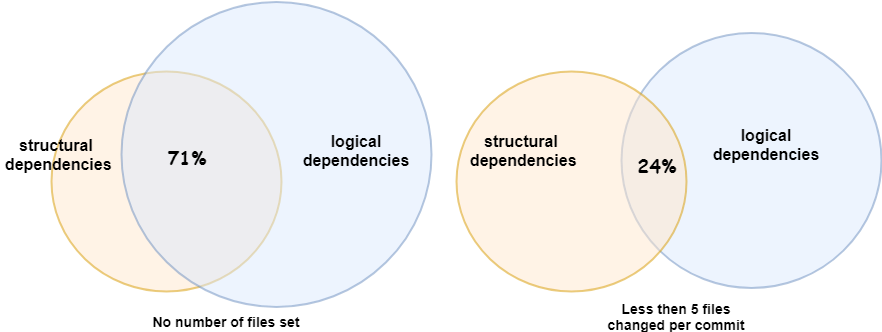
\includegraphics[scale=0.3]{fig4.png}
\caption{Venn diagrams of the overlapping rates with comments taken into consideration as change}
\label{fig:fig4}
\end{figure}


Table \ref{table:7} illustrates the percentage rates for all the categories mentioned in Subsection 2.2 and in addition a last category that takes all commits regardless of the number of changed files. How it can be seen, the overlapping rates are also influenced by the comments considerations . The rates are with aprox 6\% lower if comments are not taken into consideration as a change. 


\begin{table}[h]
  \centering
  \begin{tabular}{@{}c||cc@{}}
    \toprule
       Category & With comments & Without comments  \\
    \midrule
less 5	&	24.33\% &	17,4\%	\\
more 5 less 20	&	36.26\% &	32,81\%\\
more 20	&	35.33\%	&	34,89\%\\
total & 71,47\% & 64.9\% \\
    \bottomrule
  \end{tabular}
  \caption{ overall percentage rates }
   \label{table:7}
\end{table}

As a conclusion, it results large number of structural dependencies are not doubled by logical which can indicate that the systems are stable. It also result that taken or not comments as change, the final results are not influenced in a big percentage. What influences the result of the overlaping between logical and structural dependencies is the number of files taken into consideration .


\begin{thebibliography}{1}

\bibitem{ct1}
David Binkley, \emph{Source Code Analysis: A Road Map}, Future of Software Engineering, 2007. FOSE '07.
\bibitem{ct8}
N. Ajienka and A. Capiluppi, \emph{Understanding the interplay between the logical and structural coupling of software classes}, J. Systems Software, vol. 134, pp. 120-137, 2017.
\bibitem{ct6}
Igor Wiese, Rodrigo Kuroda, Reginaldo Re, Gustavo Oliva, Marco Gerosa, \emph{An Empirical Study of the Relation Between Strong Change Coupling and Defects Using History and Social Metrics in the Apache Aries Project}, IFIP International Conference on Open Source Systems, OSS 2015: Open Source Systems: Adoption and Impact, pp. 3-12.
\bibitem{ct2}
G. Booch, \emph{Object-Oriented Analysis and Design with Applications}, Third Edition: Addison-Wesley, 2007.
\bibitem{ct3}
Marcelo Cataldo, Audris Mockus, Jeffrey A. Roberts, and James D. Herbsleb, \emph{Software Dependencies, Work Dependencies, and Their Impact on Failures},  IEEE Transactions on Software Engineering ( Volume: 35, Issue: 6, Nov.-Dec. 2009 ), pp. 864-878.
\bibitem{ct4}
Beck F., Diehl S.,\emph{ On the congruence of modularity and code coupling}, In ESEC/FSE'11: European Software Engineering Conference and Symposium on Foundations of Software Engineering (2011), pp. 354-364.
\bibitem{ct5}
Liguo Yu,\emph{Understanding component co-evolution with a study on Linux}, Empirical Software Engineering, April 2007, Volume 12, Issue 2, pp. 123-141.
\bibitem{ct7}
 Ben Collins-Sussman, Brian W. Fitzpatrick, and C. Michael Pilato, \emph{Version Control with Subversion}, http://svnbook.red-bean.com/en/1.7/svn.basic.version-control-basics.html, 2008.
\bibitem{ct9}
 Huzefa Kagdi, Malcom Gethers, Denys Poshyvanyk, Michael L. Collard,\emph{Blending Conceptual and Evolutionary Couplings to Support Change Impact Analysis in Source Code}, 17th Working Conference on IEEE, 2010, pp. 119-128.
\bibitem{ct10}
Poshyvanyk, Denys, \emph{Using information retrieval based coupling measures for impact analysis}, Empirical Software Engineering 14 ,2008, pp. 5-32.

\end{thebibliography}


\end{document}










